%\documentstyle[epsf,twocolumn]{jarticle}       %LaTeX2.09�d�l
\documentclass[twocolumn]{jarticle} 
%%%%%%%%%%%%%%%%%%%%%%%%%%%%%%%%%%%%%%%%%%%%%%%%%%%%%%%%%%%%%%
%%
%%  n�{ �o�[�W����
%%
%%%%%%%%%%%%%%%%%%%%%%%%%%%%%%%%%%%%%%%%%%%%%%%%%%%%%%%%%%%%%%%%
\setlength{\topmargin}{-45pt}
%\setlength{\oddsidemargin}{0cm} 
\setlength{\oddsidemargin}{-7.5mm}
%\setlength{\evensidemargin}{0cm} 
\setlength{\textheight}{24.1cm}
%setlength{\textheight}{25cm} 
\setlength{\textwidth}{17.4cm}
%\setlength{\textwidth}{172mm} 
\setlength{\columnsep}{11mm}


%�y�߂������邲�Ƃ�(1.1)(1.2) �c(2.1)(2.2)�Ɛ����ԍ����‚����Ƃ��z
%\makeatletter
%\renewcommand{\theequation}{%
%\thesection.\arabic{equation}} %\@addtoreset{equation}{section}
%\makeatother

%\renewcommand{\arraystretch}{0.95} �sT�̐ݒ�

%%%%%%%%%%%%%%%%%%%%%%%%%%%%%%%%%%%%%%%%%%%%%%%%%%%%%%%%
\usepackage[dvipdfmx]{graphicx}  %pLaTeX2e�d�l(�v\documentstyle ->\documentclass)
\usepackage{bm}
\usepackage{amsmath, amssymb}
\usepackage{enumerate}
%%%%%%%%%%%%%%%%%%%%%%%%%%%%%%%%%%%%%%%%%%%%%%%%%%%%%%%%

\begin{document}

\twocolumn[
\noindent

\hspace{1em}
令和3年7月5日(月) 2021年度前期研究発表会資料
\hfill
B4 尾關 拓巳

\vspace{2mm}

\hrule

\begin{center}
{\Large \bf 進化型計算および Nelder-Mead 法によるエネルギープラント運用計画の\\最適化}
\end{center}


\hrule
\vspace{3mm}
]

\section{はじめに}
エネルギープラントは工場や建物全体におけるエネルギー消費の大部分を占めており,エネルギー管理者にとってエネルギープラントの省エネルギー化は優先的に取り組むべき課題である.エネルギープラントの効率的な省エネルギー手法として,エネルギーマネジメントシステム(EMS)が適用されている.しかしながら EMS を適用するにあたっては,定式化する際のモデルと実際の機器との乖離や,未だ実用的規模のプラントに対する有効な最適化技術がない等,多くの課題がある.現実のエネルギープラントの最適化は困難であるためベンチマーク問題が提案されている.

一方で,生物の進化から着想を得た確率的探索手法である進化型計算(Evolutionary Computation: EC)は,その汎用性の高さから科学や工学の様々な分野で用いられている.

本研究では,実数値最適化問題を解くための有力な EC のアルゴリズムである CMA-ES と多次元の非線形最適化問題に適用可能な局所的探索手法である Nelder-Mead 法を用いて,エネルギープラントの様々な制約条件に柔軟に対応しながら最適化できる手法の構築を目的とする.


\section{要素技術}
    \subsection{エネルギープラント問題}
    エネルギープラントでは,ガスタービン,ボイラ,冷凍機など様々な機器を用いて,電力・熱・蒸気などのエネルギーを供給している.エネルギープラント運用計画問題は,各エネルギーの需給バランス,機器の機械的制約,および運用制約を考慮したうえで,電力購入コストとガス購入コストを最小にするような機器の運転状態を計画する問題である.図\ref{energy_plant}に本研究で用いるベンチマーク問題のエネルギープラントの模式図を示す \cite{denki}.
    \begin{figure*}[hbtp]
        \centering
        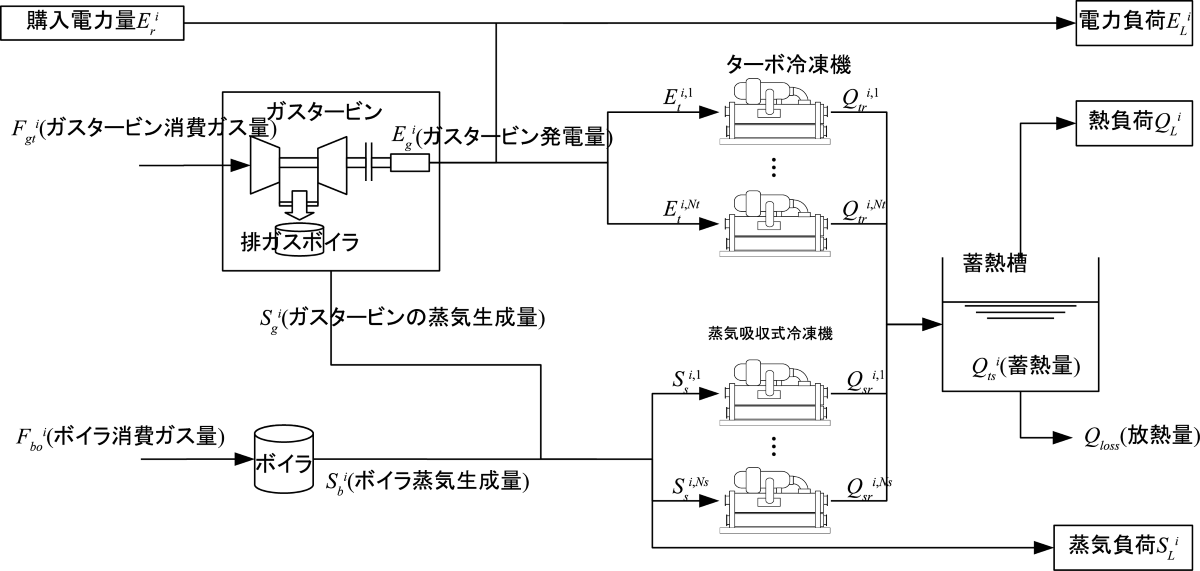
\includegraphics[keepaspectratio, scale=0.7]
            {energy_plant.png}
        \caption{エネルギープラントの模式図(文献\cite{denki}の図3.2.1参照)}
        \label{energy_plant}
       \end{figure*}
    この問題はガスタービン一台,ボイラ一台,ターボ式冷凍機一台,蒸気吸収式冷凍機二台の 5 つの機器からなる 24 時刻運用問題である.求める目的関数は 24 時刻の各時間帯で購入された電力およびガスの購入費用であり,
    \begin{equation}
        \label{fitness}
        \sum_{i=1}^I\left\{C_{E_r}^iE_r^i(x_g^i, x_t^i) + C_{F_r}^i(x_g^i + x_b^i)\right\}
    \end{equation}
    と表される.ここで,$C_{E_r}^i$ は時刻 $i$ における電力購入単価,$C_{F_r}^i$ は時刻 $i$ におけるガス購入単価,$x_g^i$ は時刻 $i$ におけるガスタービンのガス消費量,$x_t^i$ は時刻 $i$ におけるターボ式冷凍機の熱生成量,$x_b^i$ は時刻 $i$ におけるボイラのガス消費量を表す.$E_r^i$ は時刻 $i$ における電力購入量であり,
    \begin{equation}
        \label{E_r}
        E_r^i(x_g^i, x_t^i) = \sum_{j=1}^{N_t}(a_{tj}x_{tj}^i)+\bar{E}_L^i-a_{ge}x_g^i+E_{rm}^i
    \end{equation}
    と表される.ここで,$N_t$ はターボ式冷凍機の数,$a_{tj}$は,$j$ 番目のターボ式冷凍機のパラメータ,$a_{ge}$ はガスタービンのパラメータ,$x_{tj}^i$ は 時刻 $i$ における $j$ 番目のターボ式冷凍機の熱生成量,$\bar{E}_L^i$ は時刻 $i$ における電力負荷,$E_{rm}^i$ は時刻 $i$ における電力の残りを表す.

    また,起動・停止状態は二時間以上継続しなければ状態を変えられないことや動作している機器の出力の上下限制約など制約条件の詳細は,文献\cite{denki}を参照されたい.

    本問題は,240 個の変数と 423 個の制約条件を有する大規模な混合整数非線形計画問題として定式化される.決定変数に整数を含む混合整数計画問題であり,目的関数および制約条件に非線形なものを含む非線形計画問題でもあるため,最適解を探索することが困難な問題である.
    
    \subsection{Nelder-Mead 法}
    Nelder-Mead法\cite{10.1093/comjnl/7.4.308}は制約条件がない最適化問題
    \begin{equation}
        \label{minfx}
        \min f(\bm{x})
    \end{equation}
    を解くために用いられる局所探索手法である.%\cite{gao2012implementing}
    ここで,$n$ は $\bm{x}$ の次元数, $f: \mathbb{R}^n \rightarrow \mathbb{R}$ は目的関数を表す.$n$ 次元の空間で $n+1$ 個の頂点からなる単体(シンプレックス)を変形・移動する操作をしながら解を探索する.ここで,頂点 $\bm{x}_1, \bm{x}_2, \dots , \bm{x}_{n+1}$ を持つ単体を $\Delta$ と表記する. 
    
    Nelder-Mead 法は一連の単体を反復的に生成して(\ref{minfx})式の最適点を近似する.各試行で単体の頂点 $\{\bm{x}_j\}_{j=1}^{n+1}$ を(\ref{orderdfx})式のように目的関数値に従って順序付ける.
    \begin{equation}
        \label{orderdfx}
        f(\bm{x}_1) \leq f(\bm{x}_2) \leq \cdots \leq f(\bm{x}_{n+1})
    \end{equation}
    ただし$\bm{x}_1$ を最良な頂点,$\bm{x}_{n+1}$ を最悪の頂点とする.

    アルゴリズムで用いる単体の操作には反射,拡大,収縮,縮小があり,それぞれにスカラー値のパラメーター $\alpha$ (反射), $\beta$ (拡大), $\gamma$ (収縮),$\delta$ (縮小) が与えられている.ただし,パラメータの値は,$\alpha > 0$, $\beta > 1$, $0 < \gamma < 1$, $0 < \delta < 1$ を満たす.Nelder-Mead 法の標準的な実装ではパラメーターは(\ref{parameters})式のように選ばれている.
    \begin{equation}
        \label{parameters}
        \{\alpha, \beta, \gamma, \delta\} = \{1, 2, 0.5, 0.5\}
    \end{equation}
    
    目的関数が小さい順で $n$ 番目までの頂点の重心 $\bar{\bm{x}}$ は,(\ref{centroid})式で表される.
    \begin{equation}
        \label{centroid}
        \bar{\bm{x}} = \frac{1}{n}\sum_{i=1}^n\bm{x}_i
    \end{equation}

    ここで,Nelder-Mead 法での 1 試行のアルゴリズムの概要を述べる.
    \begin{enumerate}[Step 1]
        \item \textbf{ソート}: $\Delta$ の $n+1$ 個の頂点を $f$ で評価し,(\ref{orderdfx})式が成立するようにソートする.
        \item \textbf{反射}: 反射点 $\bm{x}_\mathrm{r}$ を(\ref{x_r})式で計算する.
        \begin{equation}
            \label{x_r}
            \bm{x}_\mathrm{r} = \bar{\bm{x}} + \alpha(\bar{\bm{x}} - \bm{x}_{n+1})
        \end{equation}
        $f_\mathrm{r} = f(\bm{x}_\mathrm{r})$ を評価する.もし$f_1 \leq f_\mathrm{r} < f_n$ であれば,$\bm{x}_{n+1}$ を $\bm{x}_\mathrm{r}$ に置き換える.
        \item \textbf{拡大}: もし$f_\mathrm{r} < f_1$ であれば,(\ref{x_e})式で拡大点 $\bm{x}_\mathrm{e}$ を計算し,$f_\mathrm{e} = f(\bm{x}_\mathrm{e})$ を評価する.
        \begin{equation}
            \label{x_e}
            \bm{x}_\mathrm{e} = \bar{\bm{x}} + \beta(\bm{x}_\mathrm{r} - \bar{\bm{x}})
        \end{equation}
        $f_\mathrm{e} < f_\mathrm{r}$ のとき,$\bm{x}_{n+1}$ を $\bm{x}_\mathrm{e}$ に置き換える.そうでなければ,$\bm{x}_{n+1}$ を $\bm{x}_\mathrm{r}$ に置き換える.
        \item \textbf{外側の収縮}: もし$f_n \leq f_\mathrm{r} < f_{n+1}$ であれば,(\ref{x_oc})式で外側の収縮点 $\bm{x}_\mathrm{oc}$ を計算し,$f_\mathrm{oc} = f(\bm{x}_\mathrm{oc})$ を評価する.
        \begin{equation}
            \label{x_oc}
            \bm{x}_\mathrm{oc} = \bar{\bm{x}} + \gamma(\bm{x}_\mathrm{r} - \bar{\bm{x}})
        \end{equation}
        $f_\mathrm{oc} \leq f_\mathrm{r}$ のとき, $\bm{x}_{n+1}$ を $\bm{x}_\mathrm{oc}$ に置き換える.そうでなければ,Step 6に移行する.
        \item \textbf{内側の収縮}: もし $f_\mathrm{r} \geq f_{n+1}$ であれば,(\ref{x_ic})式で内側の収縮点 $\bm{x}_\mathrm{ic}$ を計算し,$f_\mathrm{ic} = f(\bm{x}_\mathrm{ic})$ を評価する.
        \begin{equation}
            \label{x_ic}
            \bm{x}_\mathrm{ic} = \bar{\bm{x}} - \gamma(\bm{x}_\mathrm{r} - \bar{\bm{x}})
        \end{equation}
        $f_\mathrm{ic} < f_{n+1}$ のとき,$\bm{x}_{n+1}$ を $\bm{x}_\mathrm{ic}$ に置き換える.そうでなければ,Step 6 に移行する.
        \item \textbf{縮小}: $2 \leq i \leq n+1$ に対し,(\ref{x_i})式を計算する.
        \begin{equation}
            \label{x_i}
            \bm{x}_\mathrm{i} = \bm{x}_1 + \delta(\bm{x}_\mathrm{i} - \bm{x}_1)
        \end{equation}
    \end{enumerate}

    \subsection{CMA-ES}
    進化型計算のひとつである共分散行列進化適応戦略(Evolution Strategy with Covarience Matrix Adaptation, CMA-ES)%\cite{542381}
    は悪スケール性や変数間依存といった最適化を困難にする特徴を持つ実数値最適化問題に対する有力なアルゴリズムである.%\cite{akimoto2016}
    CMA-ES による探索では個体は多変量正規分布を用いた突然変異により生成される.この多変量生成分布の統計量である平均ベクトルおよび共分散行列を更新していくことで,探索を進める.

\section{問題設定}
ガスタービン一台,ボイラ一台,ターボ式冷凍機一台,蒸気吸収式冷凍機二台の5つの機器からなる 24 時刻運用問題である.入力変数は各機器の熱生成量またはガス消費量を表す $\bm{x}$ と 2 値で各機器の稼働状態表す $\bm{y}$ が存在し,どちらも120次元である.表\ref{explain_variables}に各機器の熱生成量またはガス消費量の上下限値を示す.なお,各機器が停止状態のときは 0 となる.
\begin{table}[hbtp]
    \caption{各機器のガス消費量または熱生成量の上下限値}
    \label{explain_variables}
    \centering
    \begin{tabular}{|c|c|c|}
        \hline
        ガス消費量または熱生成量 & 上限値 & 下限値  \\
        \hline
        ターボ式冷凍機の熱生成量 & 1.5 & 5.0  \\
        蒸気吸収式冷凍機1の熱生成量 & 4.5 & 15.0  \\
        蒸気吸収式冷凍機2の熱生成量 & 4.5 & 15.0  \\
        ガスタービンのガス消費量 & 1103 & 3679 \\
        ボイラのガス消費量 & 8.02 & 803 \\
        \hline
    \end{tabular}
  \end{table}
  
\section{提案手法}
今回は Nelder-Mead 法と CMA-ES を用いた電力プラントの最適化の第一段階として,エネルギープラント運用計画のための最適化ベンチマーク問題 ver.1\cite{denki}を対象とする.なお,CMA-ES としては deap の cma の Strategy を使用した.%\cite{DEAP_JMLR2012}

単目的最適化の場合(Strategy)は(\ref{fitness})式で述べた元の目的関数を $f$, 機器の上下限制約,起動・停止状態などの満たすべき等式・不等式をまとめた制約違反関数を $V$, ペナルティ関数の係数を $\rho$ とすると, Nelder-Mead 法および CMA-ES 上での目的関数 $F$ は(\ref{F})式で表される.
\begin{equation}
    \label{F}
    F = f + \frac{\rho V}{V-V_\mathrm{th}}\max(V-V_\mathrm{th}, 0)
\end{equation}
ただし,今回の実験では制約違反関数 $V$ が制約違反関数の閾値 $V_\mathrm{th} = 1.0 \times 10^{-10}$ より小さい解を実行可能解と定義する.

予備実験により,Nelder-Mead 法はそのまま適用しても $F$ を十分に小さくできないことがわかったため,決定変数の一部である $\bm{x}$ を固定し,$\bm{y}$ のみの探索をした.$x_i(i=1,\dots,120)$ は $y_i=0$ ,すなわち機器が停止状態のときは 0, そうでないときは各上下限値の平均値とした.そして,Nelder-Mead 法で見つかった最後の解を CMA-ES の初期平均ベクトルとし,初期個体群に加えた.

Nelder-Mead 法では各値が離散値である $\bm{y}$ を連続変数で探索できるように,最初の単体における頂点座標の各値を0.99以上1.01以下のランダムな実数と設定して探索し,目的関数内で各値が 1 より小さければ 0, そうでないとき 1,と処理した後に評価した.

CMA-ES では $f$ が定めた閾値 $t$ より小さくなった場合に $F$ にペナルティを与えることで,$\rho$ を小さくしても探索中に目的関数が小さくなりすぎて実行不可能な領域を探索することを防いだ.

\section{実験}
表\ref{setting_nelder}にNelder-Mead 法で用いた実験パラメータを,表\ref{setting_cmaes}に CMA-ES で用いた実験パラメータを示す.閾値 $t$ は, Nelder-Mead 法により $\{f, V\}=\{3999381.510, 99.58317874\}$ が得られ,実行可能解の $f$ がこの付近の値となると予測したことから決定した.
\begin{table}[htbp]
    \begin{center}
        \caption{Nelder-Mead 法の実験パラメータ}
        \label{setting_nelder}
        \begin{tabular}{| c | c |} 
            \hline
            パラメータ & 値 \\ 
            \hline
            変化とみなす最小変化量 & $1.0\times10^{-5}$ \\
            変化しない場合終了するステップ数 & 200 \\
            最大試行数 & 1000 \\
            $\rho$ (ペナルティ関数の係数) & $1.0\times10^{3}$\\ 
            \hline
        \end{tabular}
    \end{center}
\end{table}

\begin{table}[htbp]
    \begin{center}
        \caption{CMA-ES の実験パラメータ}
        \label{setting_cmaes}
        \begin{tabular}{| c | c |} 
            \hline
            パラメータ & 値 \\ 
            \hline
            $\sigma$ (初期標準偏差) &  0.1 \\
            世代数 & 5000 \\
            入力変数の次元 & 120 \\
            $\lambda$ (一世代の個体数) & 1200 \\
            $\rho$ (ペナルティ関数の係数) & $1.0\times10^{4}$\\
            $t$ (閾値) & 3999000 \\
            \hline
        \end{tabular}
    \end{center}
\end{table}

表\ref{result}に実験で得た最終的な目的関数値 $f$, 制約違反関数 $V$および既知解を示す.
\begin{table}[htbp]
    \begin{center}
        \caption{実験結果}
        \label{result}
        \begin{tabular}{|c|c|c|}
            \hline
            解法 & 目的関数値 & 制約違反関数 \\ 
            \hline
            既知解1 & 3999631.278 & $2.44 \times 10^{-10}$ \\
            既知解2 & 3999635.845 & $6.43 \times 10^{-12}$ \\
            既知解3 & 4052185.662 & $3.93 \times 10^{-14}$ \\
            実験    & 4033408.653 & $9.78 \times 10^{-11}$ \\
            \hline
        \end{tabular}
    \end{center}
\end{table}
結果として既知解 3 より目的関数値が小さい実行可能解を得ることができた.

次に,図\ref{img_F}に最適化をした目的関数 $F$ の推移を,図\ref{img_f}に元の目的関数 $f$ の推移を,図\ref{img_V}に制約違反関数 $V$ の推移を示す.縦軸はそれぞれ $F, f, V$, 横軸は Nelder-Mead 法の試行数と CMA-ES の世代数である.
\begin{figure}
    \centering
    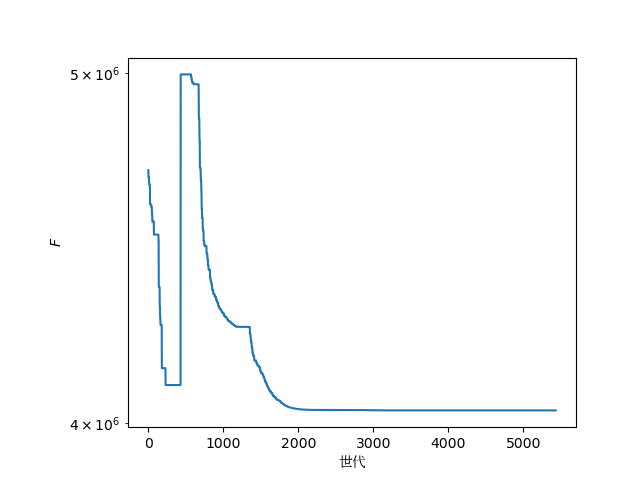
\includegraphics[width=9cm, height=7cm]{img_F.png}
    \caption{目的関数値 $F$ の推移}
    \label{img_F}
\end{figure}
\begin{figure}
    \centering
    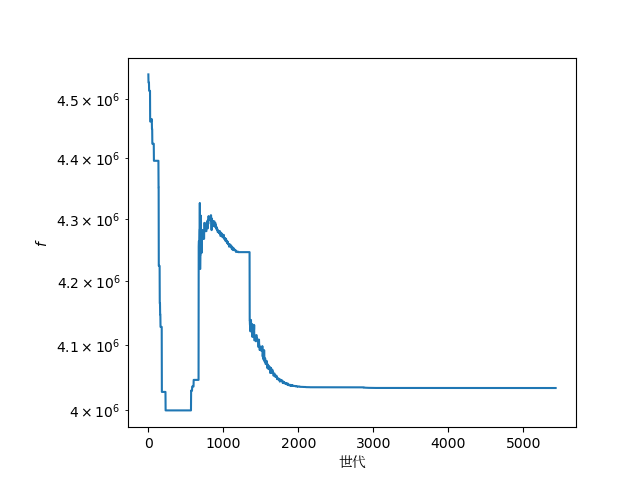
\includegraphics[width=9cm, height=7cm]{img_f.png}
    \caption{目的関数値 $f$ の推移}
    \label{img_f}
\end{figure}
\begin{figure}
    \centering
    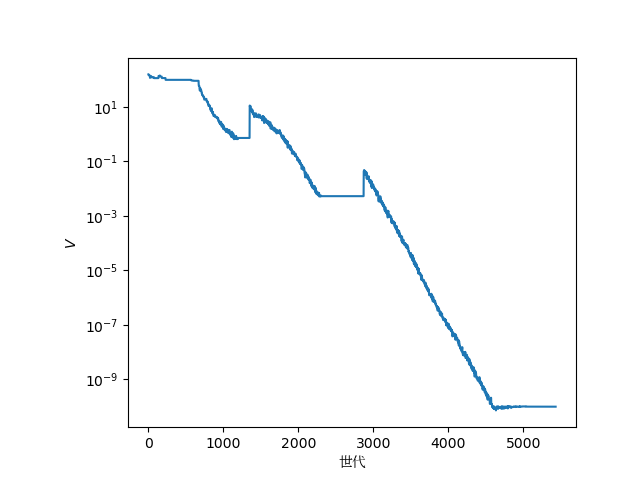
\includegraphics[width=9cm, height=7cm]{img_V.png}
    \caption{制約違反関数 $V$ の推移} 
    \label{img_V}
\end{figure}
ペナルティ関数の係数 $\rho$ が2手法間で異なり,Nelder-Mead 法は 430 試行であったため,その前後で $F$ が急に増加している.$f$ は Nelder-Mead 法で 400 万近くまで小さくできたが,その後のCMA-ESで一度 430 万程度まで増加した.また,そのときの $V$ は減少傾向にある.これは  $\rho$ が大きく, $V$ を小さくすることを優先したためだと考えられる.Nelder-Mead 法では, $V$ は最初から低く,あまり減少していない.これは $\bm{x}$ を適切な値に固定したためだと考えられる.

\section{まとめと今後の課題}
本研究では Nelder-Mead 法と CMA-ES による電力プラントの最適化について検討し,既知解に近い実行可能解を得ることができたが,最良の既知解を改善することはできなかった.今後の課題として,ペナルティ関数の係数を最適化の途中で調整することや,各手法の実験パラメータの調整があげられる.

%参考文献
\bibliographystyle{junsrt}
\bibliography{hoge} %ファイル名

\end{document}